\section{The iPhone Application}
The two main important aspect about our project was \textbf{how well the system works} and \textbf{how much easy it is to use}. For this second reason we chose to develop an application that was easy to use.\\

In order to create a mobile application that is easy to use for everyone it must focus on the final purpose, that in our case is to permit the users to check in in the lectures. That's why we create as many views as possible, letting the application do the rest.\\
We can split the behaviours manly in two set:
\begin{enumerate}
\item The single login operation (stateless)
\item The set of actions the user can do when he/she is \emph{not} inside a lecture room (\textbf{browse operations})
\item The set of action the user can do the he/she is inside the lecture room (\textbf{checkin operations})
\end{enumerate}

\subsection{The technical operation}
Of course since the application is meant to be linked to a single user is mandatory provide an authentication mechanism. Since \UB\ is also meant to work closely with the iCorsi platform we chose to use the same user account of iCorsi also for the \UB\ platform.

\begin{figure}[htbp]
\begin{center}
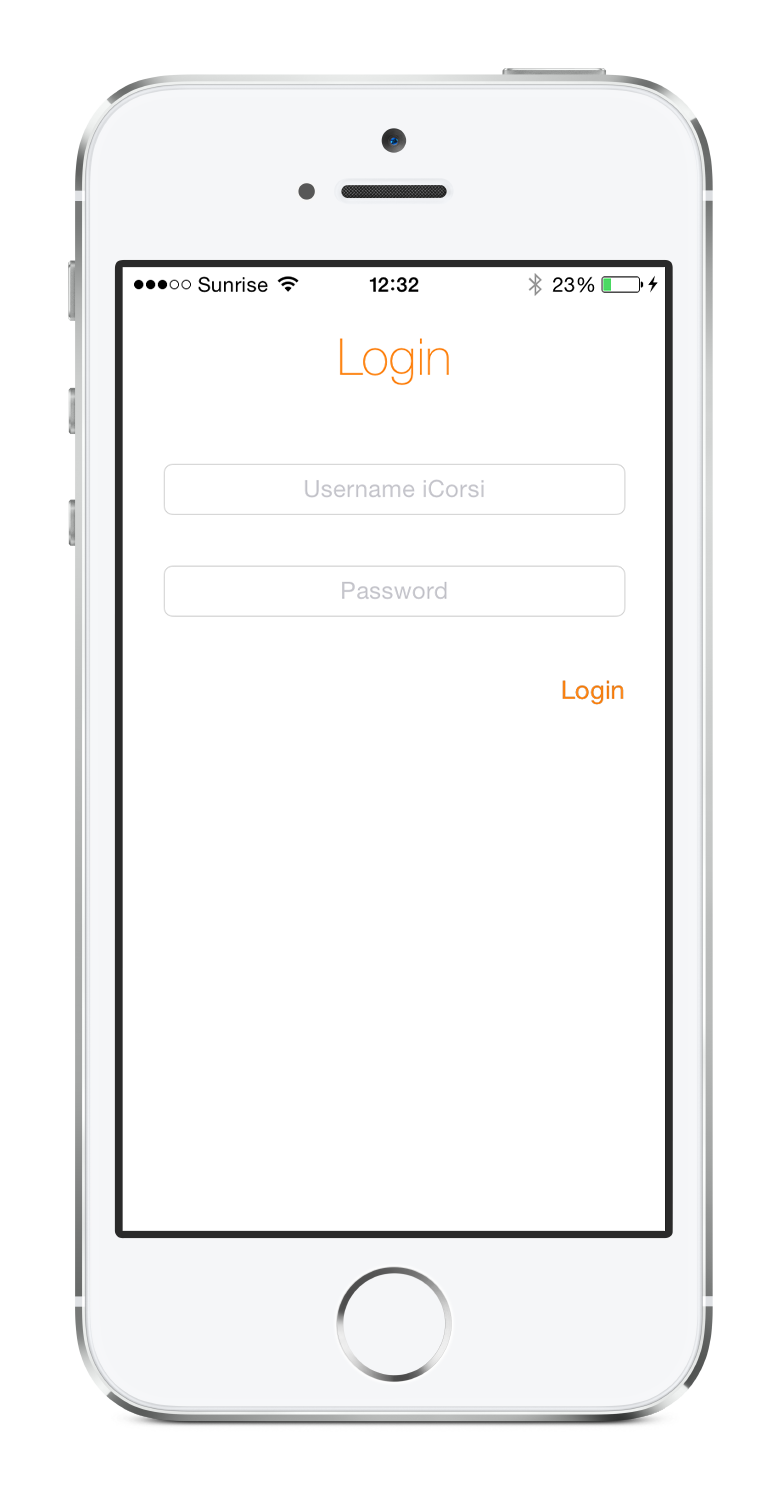
\includegraphics[scale=0.5]{img/iphone_login.png}
\caption{The login view of \UB\ }
\label{loginview}
\end{center}
\end{figure}

From then, the first technical step the user need to do is to \textbf{login} to the platform. We tried to keep the step as little as possible, saving the credential locally in the device once the login is successful.

\subsection{Outside behaviours}

The operations permitted to the user when he/she is outside the lecture room are the following:
\begin{itemize}
\item Login (stateless)
\item Search for the upcoming lectures
\item Choose the lectures he/she is going to attend
\item Start the position tracking
\item Chose a different upcoming lecture
\end{itemize}

\begin{figure}[htbp]
\begin{center}
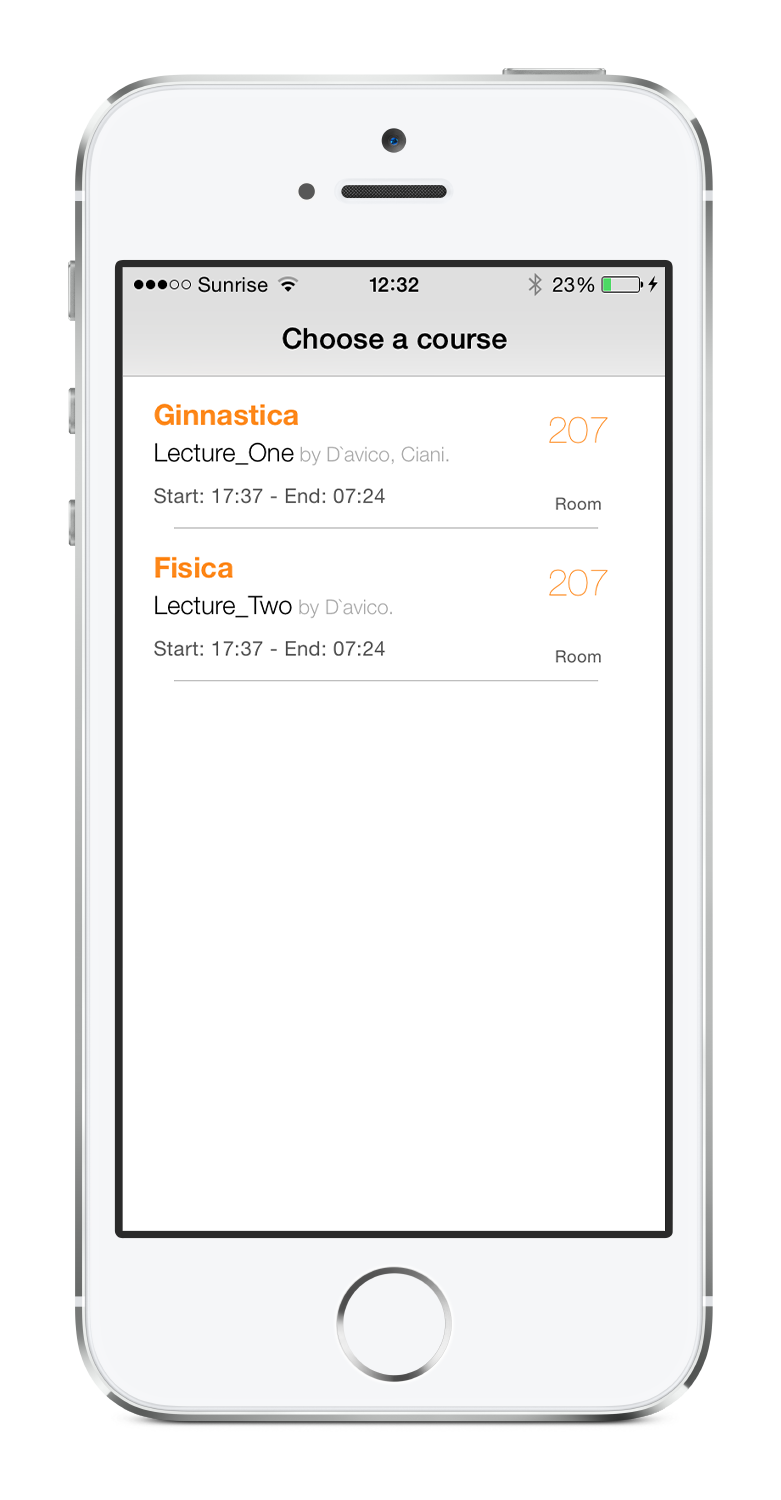
\includegraphics[scale=0.5]{img/iphone_courses.png}
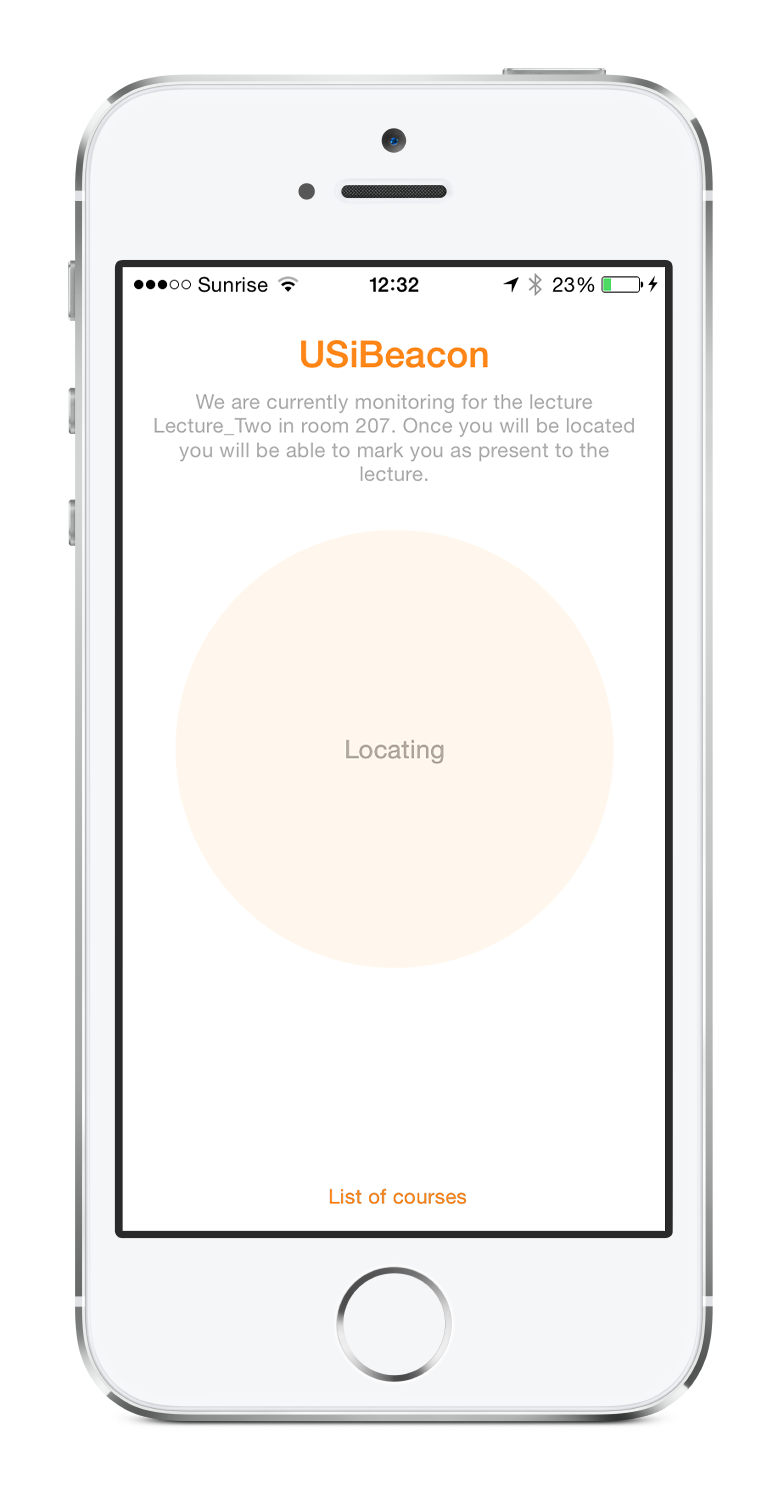
\includegraphics[scale=0.5]{img/iphone_locating.png}
\caption{The course selection (left) and the searching view (right)}
\label{courseselection}
\end{center}
\end{figure}

We chose to implement all these operation in a way that was as fast as possible: when the users open the application (and the are logged in) it automatically retrieves the list of the upcoming lectures that user should attend \textbf{within a time window of 15 minutes}.
If there is only one result the application will automatically go in ``tracking mode", starting to search for the room associated to that lecture, if instead the user has some overlaps (so there are multiple upcoming lectures) the application shows the course selection view (image \ref{courseselection} on the left) that permits the user to choose for which lecture start the tracking.\\

The last point (chose a different lecture) is achieved by a little button on the button of the searching view (image \ref{courseselection} on the right). This button permits to open again the course selection and choose a new lecture to track.

\subsection{Inside operation}
When the user move inside the room the application changes the behaviours permitting the user to \textbf{check in} to the lecture.\\

The application modifies the tracking view showing the checkin button as shown in figure \ref{checkinview}:

\begin{figure}[htbp]
\begin{center}
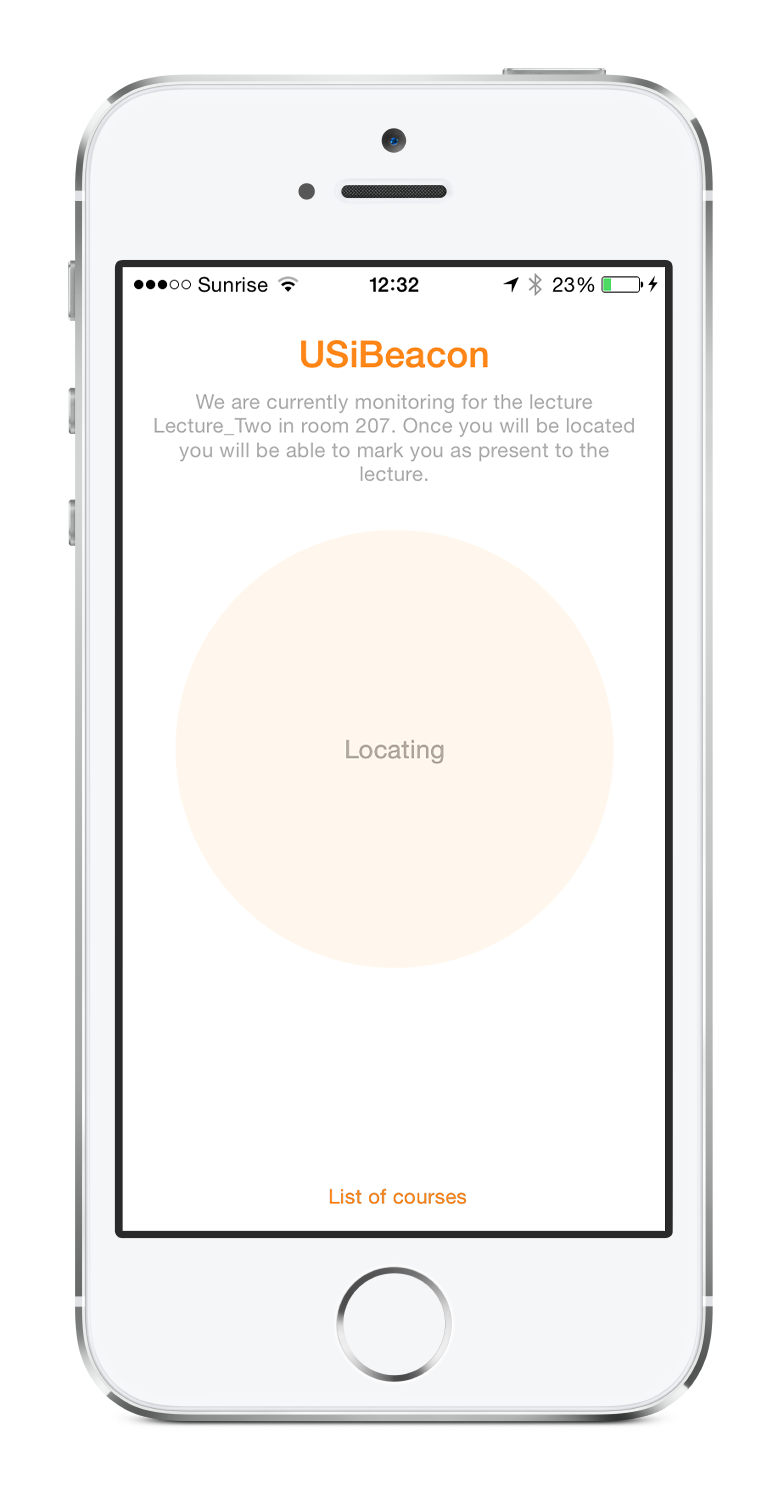
\includegraphics[scale=0.5]{img/iphone_locating.png}
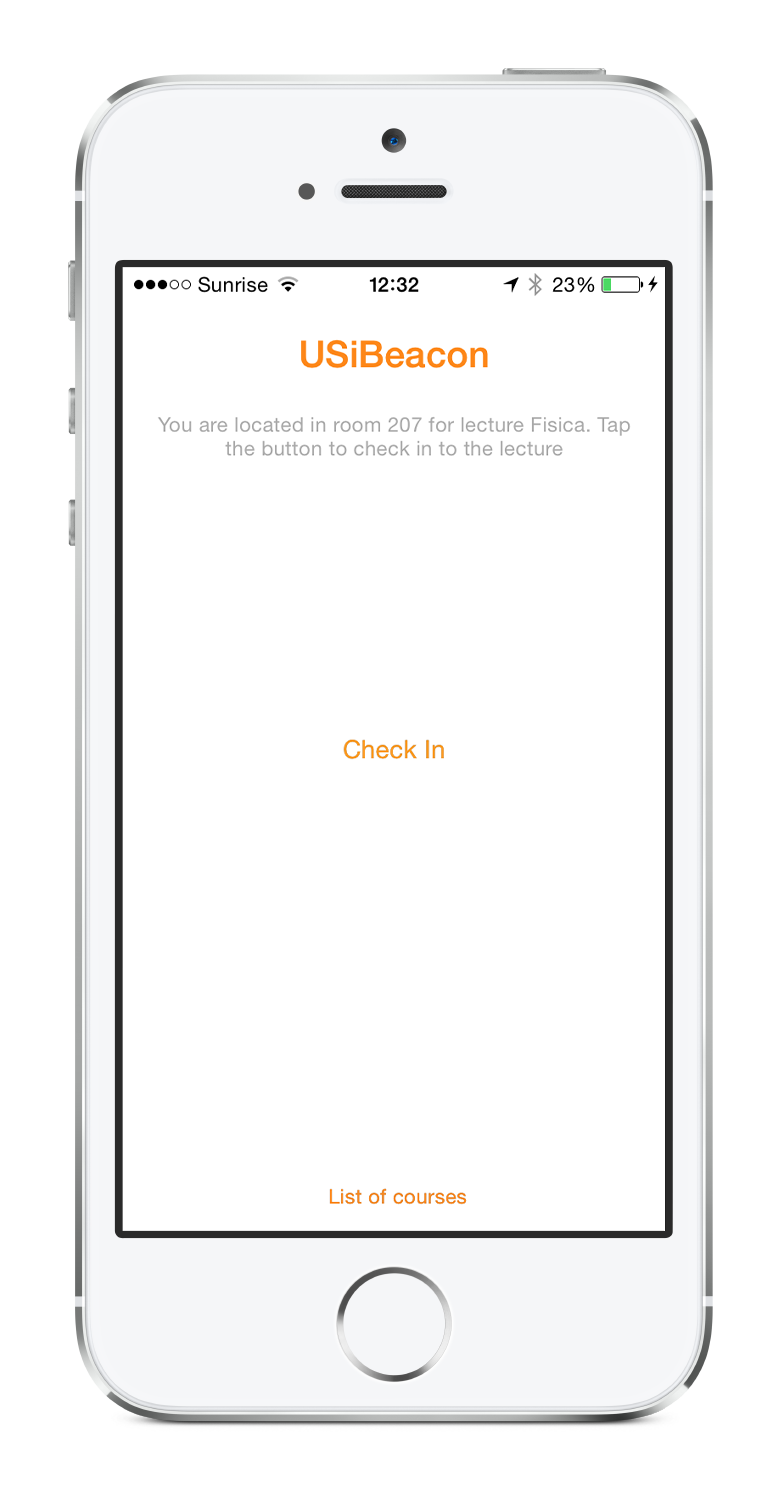
\includegraphics[scale=0.5]{img/iphone_founded.png}
\caption{The tracking view outside the room (left) and inside the tracked room (right)}
\label{checkinview}
\end{center}
\end{figure}

Once the user tap on the \emph{check in} button the application replies with the result of the checkin process that could be one of the following:
\begin{itemize}
\item \textbf{Successful:} The checkin process is concluded and the user is correctly signed to the lecture.
\item \textbf{Already Signed:} If the user tries to sign again to the same lecture a warning is visualised.
\item \textbf{Credential Error:} If the user is trying to checkin but his/her token is expired or the iCorsi password is changed an error is visualised and the user is \emph{not} signed to the lecture. In this case the login view (image \ref{loginview}) is visualised again to refresh the status.
\end{itemize}

